

\documentclass[../../e1_tp1_main.tex]{subfiles}

\begin{document}
\chapter{Curvas características}
Se busca simular las curvas características de distintos dispositivos y corroborar estas simulaciones con las mediciones obtenidas:

\begin{enumerate}
	\item Diodo común
	\item Diodo Zener
	\item Transistor bipolar
\end{enumerate}

Todas las simulaciones fueron realizadas en LTSPICE. 

\section{Curva del diodo común}
	El diodo utilizado fue el 1N4007, para el cual la tensión de breakdown es de -1000V y su tensión threshold es cercana a los 0.7 V\par
		Se utilizó una fuente de tensión continua, a la cual se la fue variando y se midió la tensión en el diodo y la corriente que circulaba por la resistencia con tester.\par
	El circuito propuesto para realizar las mediciones es el siguiente:
	
	\begin{figure}[H]	%diodo, circuito propuesto
		\centering
		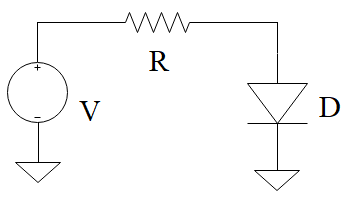
\includegraphics[scale=1.2]{imagenes/circuito_diode.png}
		\caption{Circuito propuesto para las mediciones del diodo.}
		\label{fig:ej5_circuito_diode}
	\end{figure}

	Con R = 20V.
	Las curvas resultantes de las mediciones y de las simulaciones fueron las siguientes:
\begin{figure}[H]	%diodo, curva
	\centering
	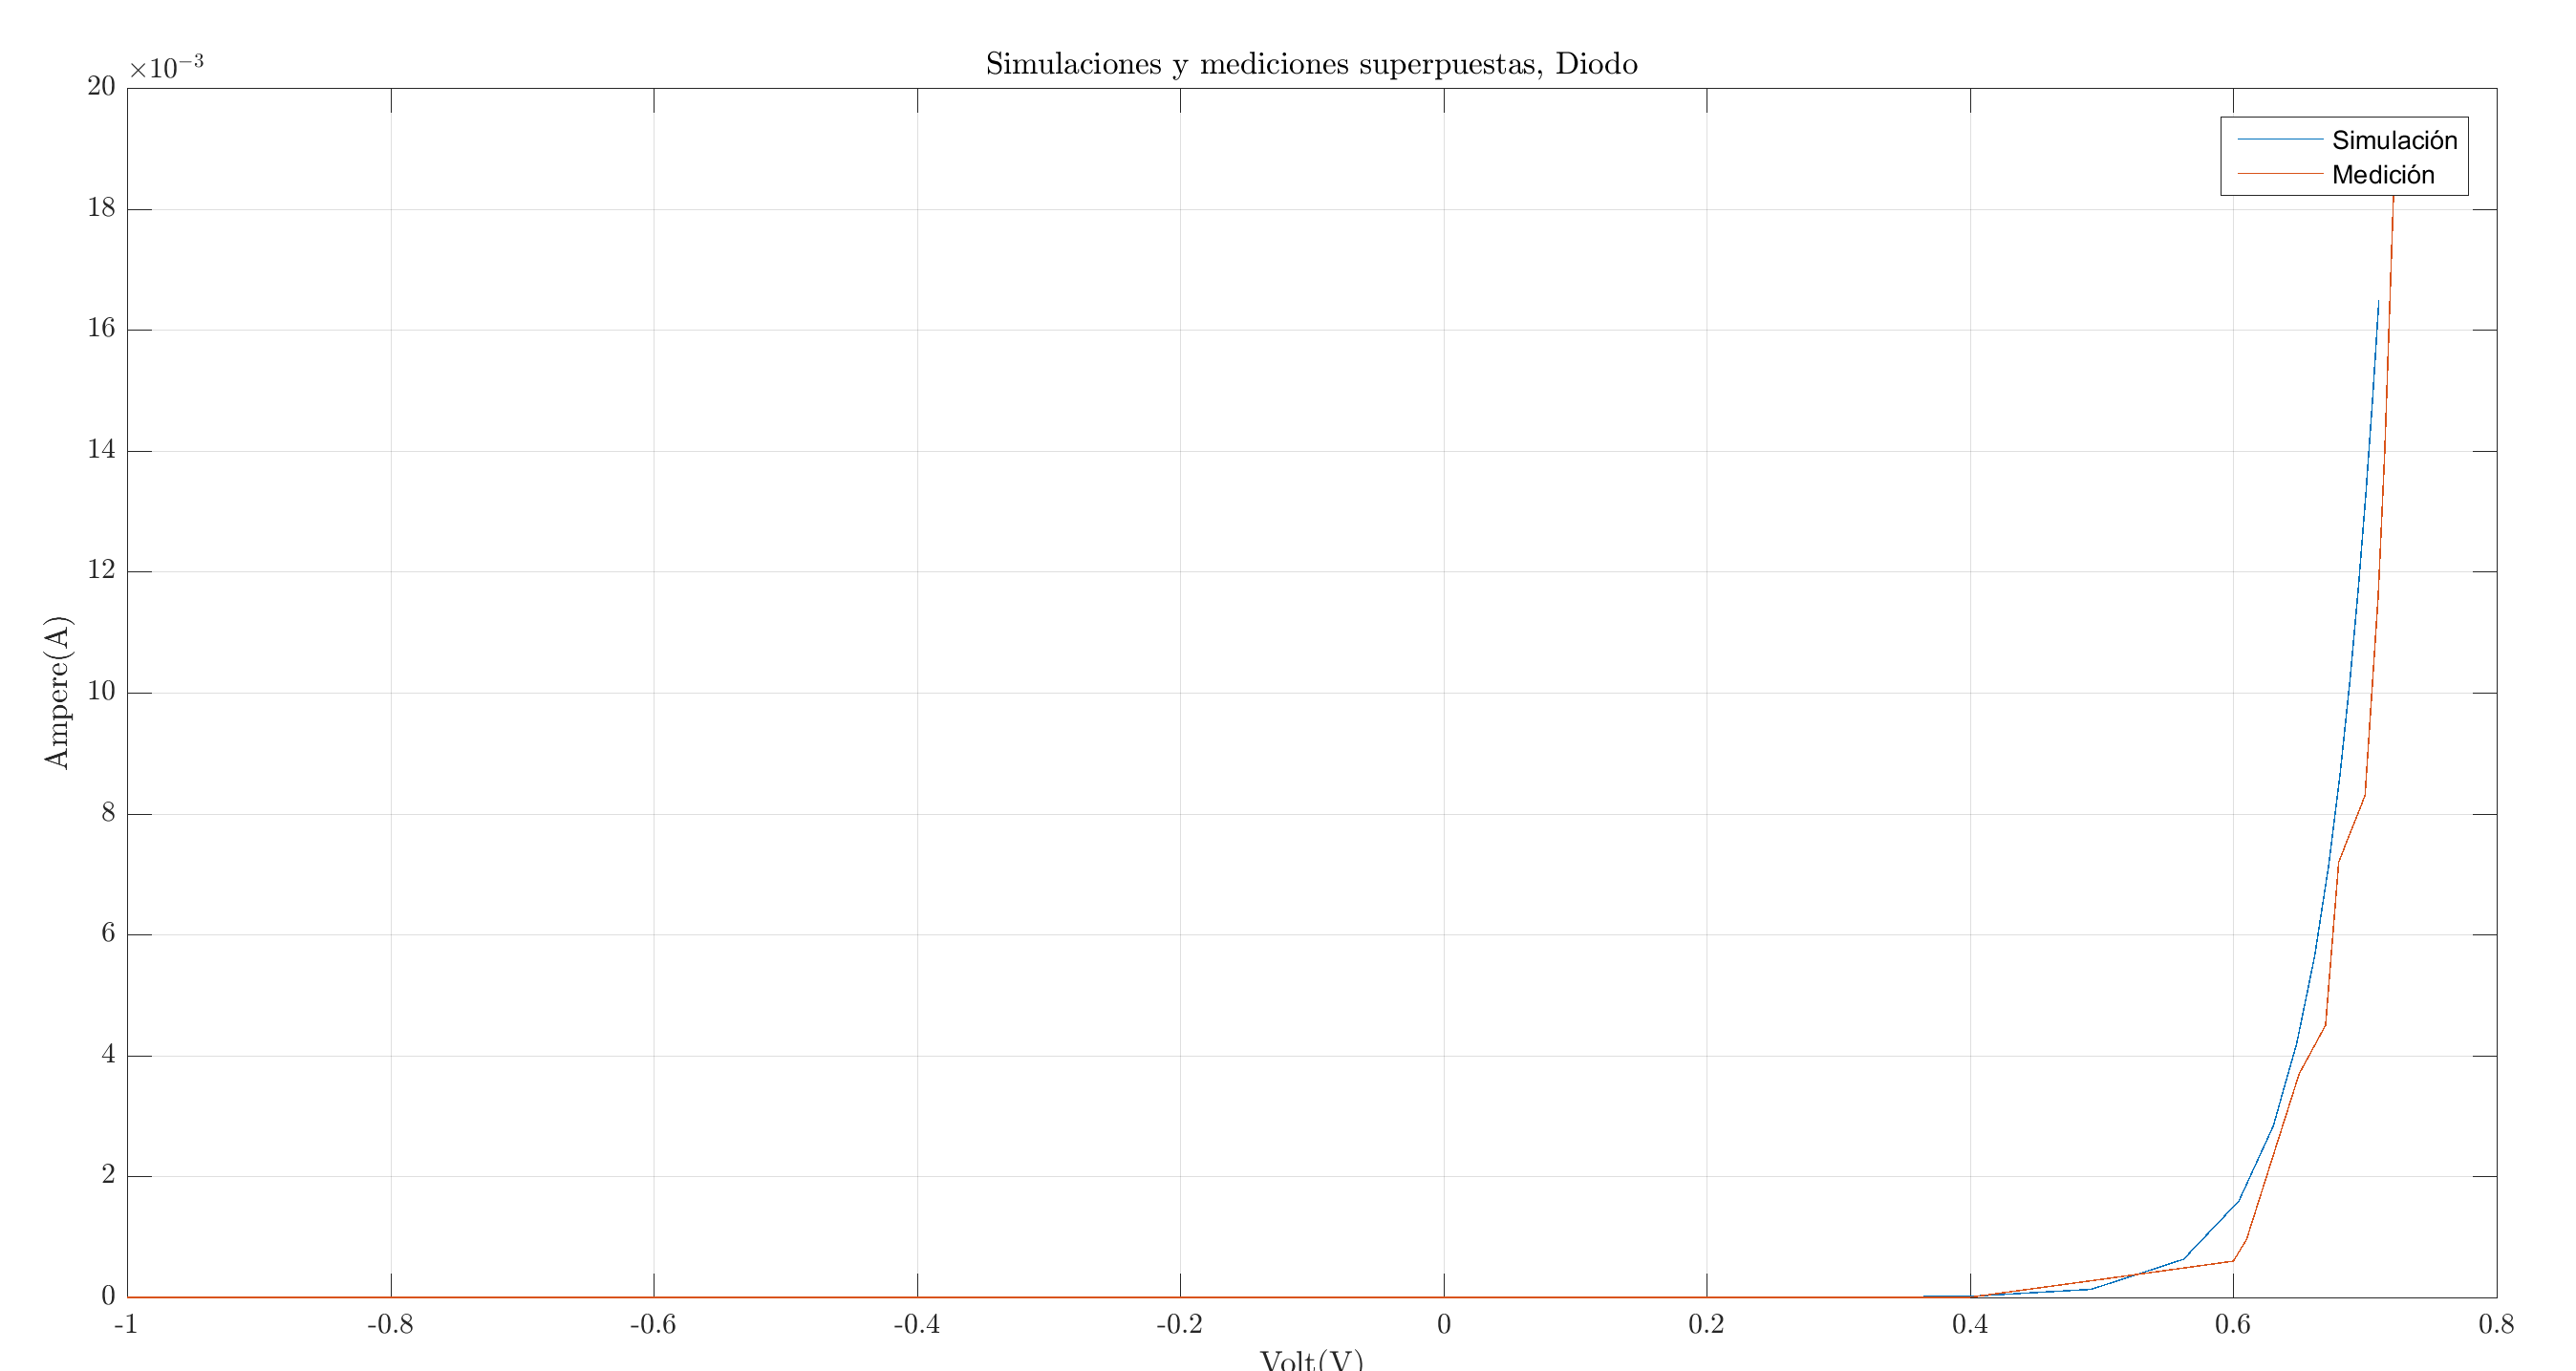
\includegraphics[scale=0.2]{imagenes/diodo_simulacion_medicion.png}
	\caption{Simulación de la curva del diodo y medición superpuestas.}
	\label{fig:ej5_diodo_simulacion_medicion}
\end{figure}

	La curva simulada coincide con la medida, por lo que se verifica que el diodo cumple con el modelo ideal.\par
	Debe hacerse notar que  la corriente en valores inferiores a los 0.3V no pudo ser medida, ya que el tester arrojaba una medición de 0V en su mínima escala. Esto se corresponde con el modelo teórico del diodo ya que la corriente en estos valores de tensión será del orden de los \micro A, medición que no podrá ser realizada con los tester del pañol.\par

\section{Curva del diodo Zener}

	El diodo Zenner utilizado fue un diodo Zener de 3,9 V, modelo 1N4730A. Sin embargo, las simluaciones en LTSPICE se hicieron con el modelo GP3V9 ya que no se pudo obtener el modelo del 1N4730A para el SPICE, por lo que se espera una diferencia entre la curva simulada y la medida.\par
	Se utilizó una fuente de tensión continua, a la cual se la fue variando y se midió la tensión en el diodo y la corriente que circulaba por la resistencia con tester.\par
	
	El circuito propuesto para realizar las mediciones es el siguiente:
	
	\begin{figure}[H]	%zener, circuito propuesto
		\centering
		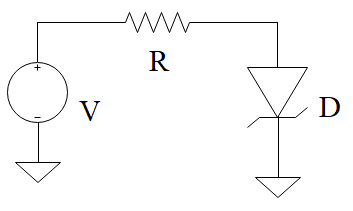
\includegraphics[scale=1.2]{imagenes/circuito_zener.png}
		\caption{Circuito propuesto para las mediciones del diodo Zener.}
		\label{fig:ej5_circuito_zener}
	\end{figure}

	Con R = 10V.
	Las curvas resultantes de las mediciones y de las simulaciones fueron las siguientes:
	 
\begin{figure}[H]	%zener, curva
	\centering
	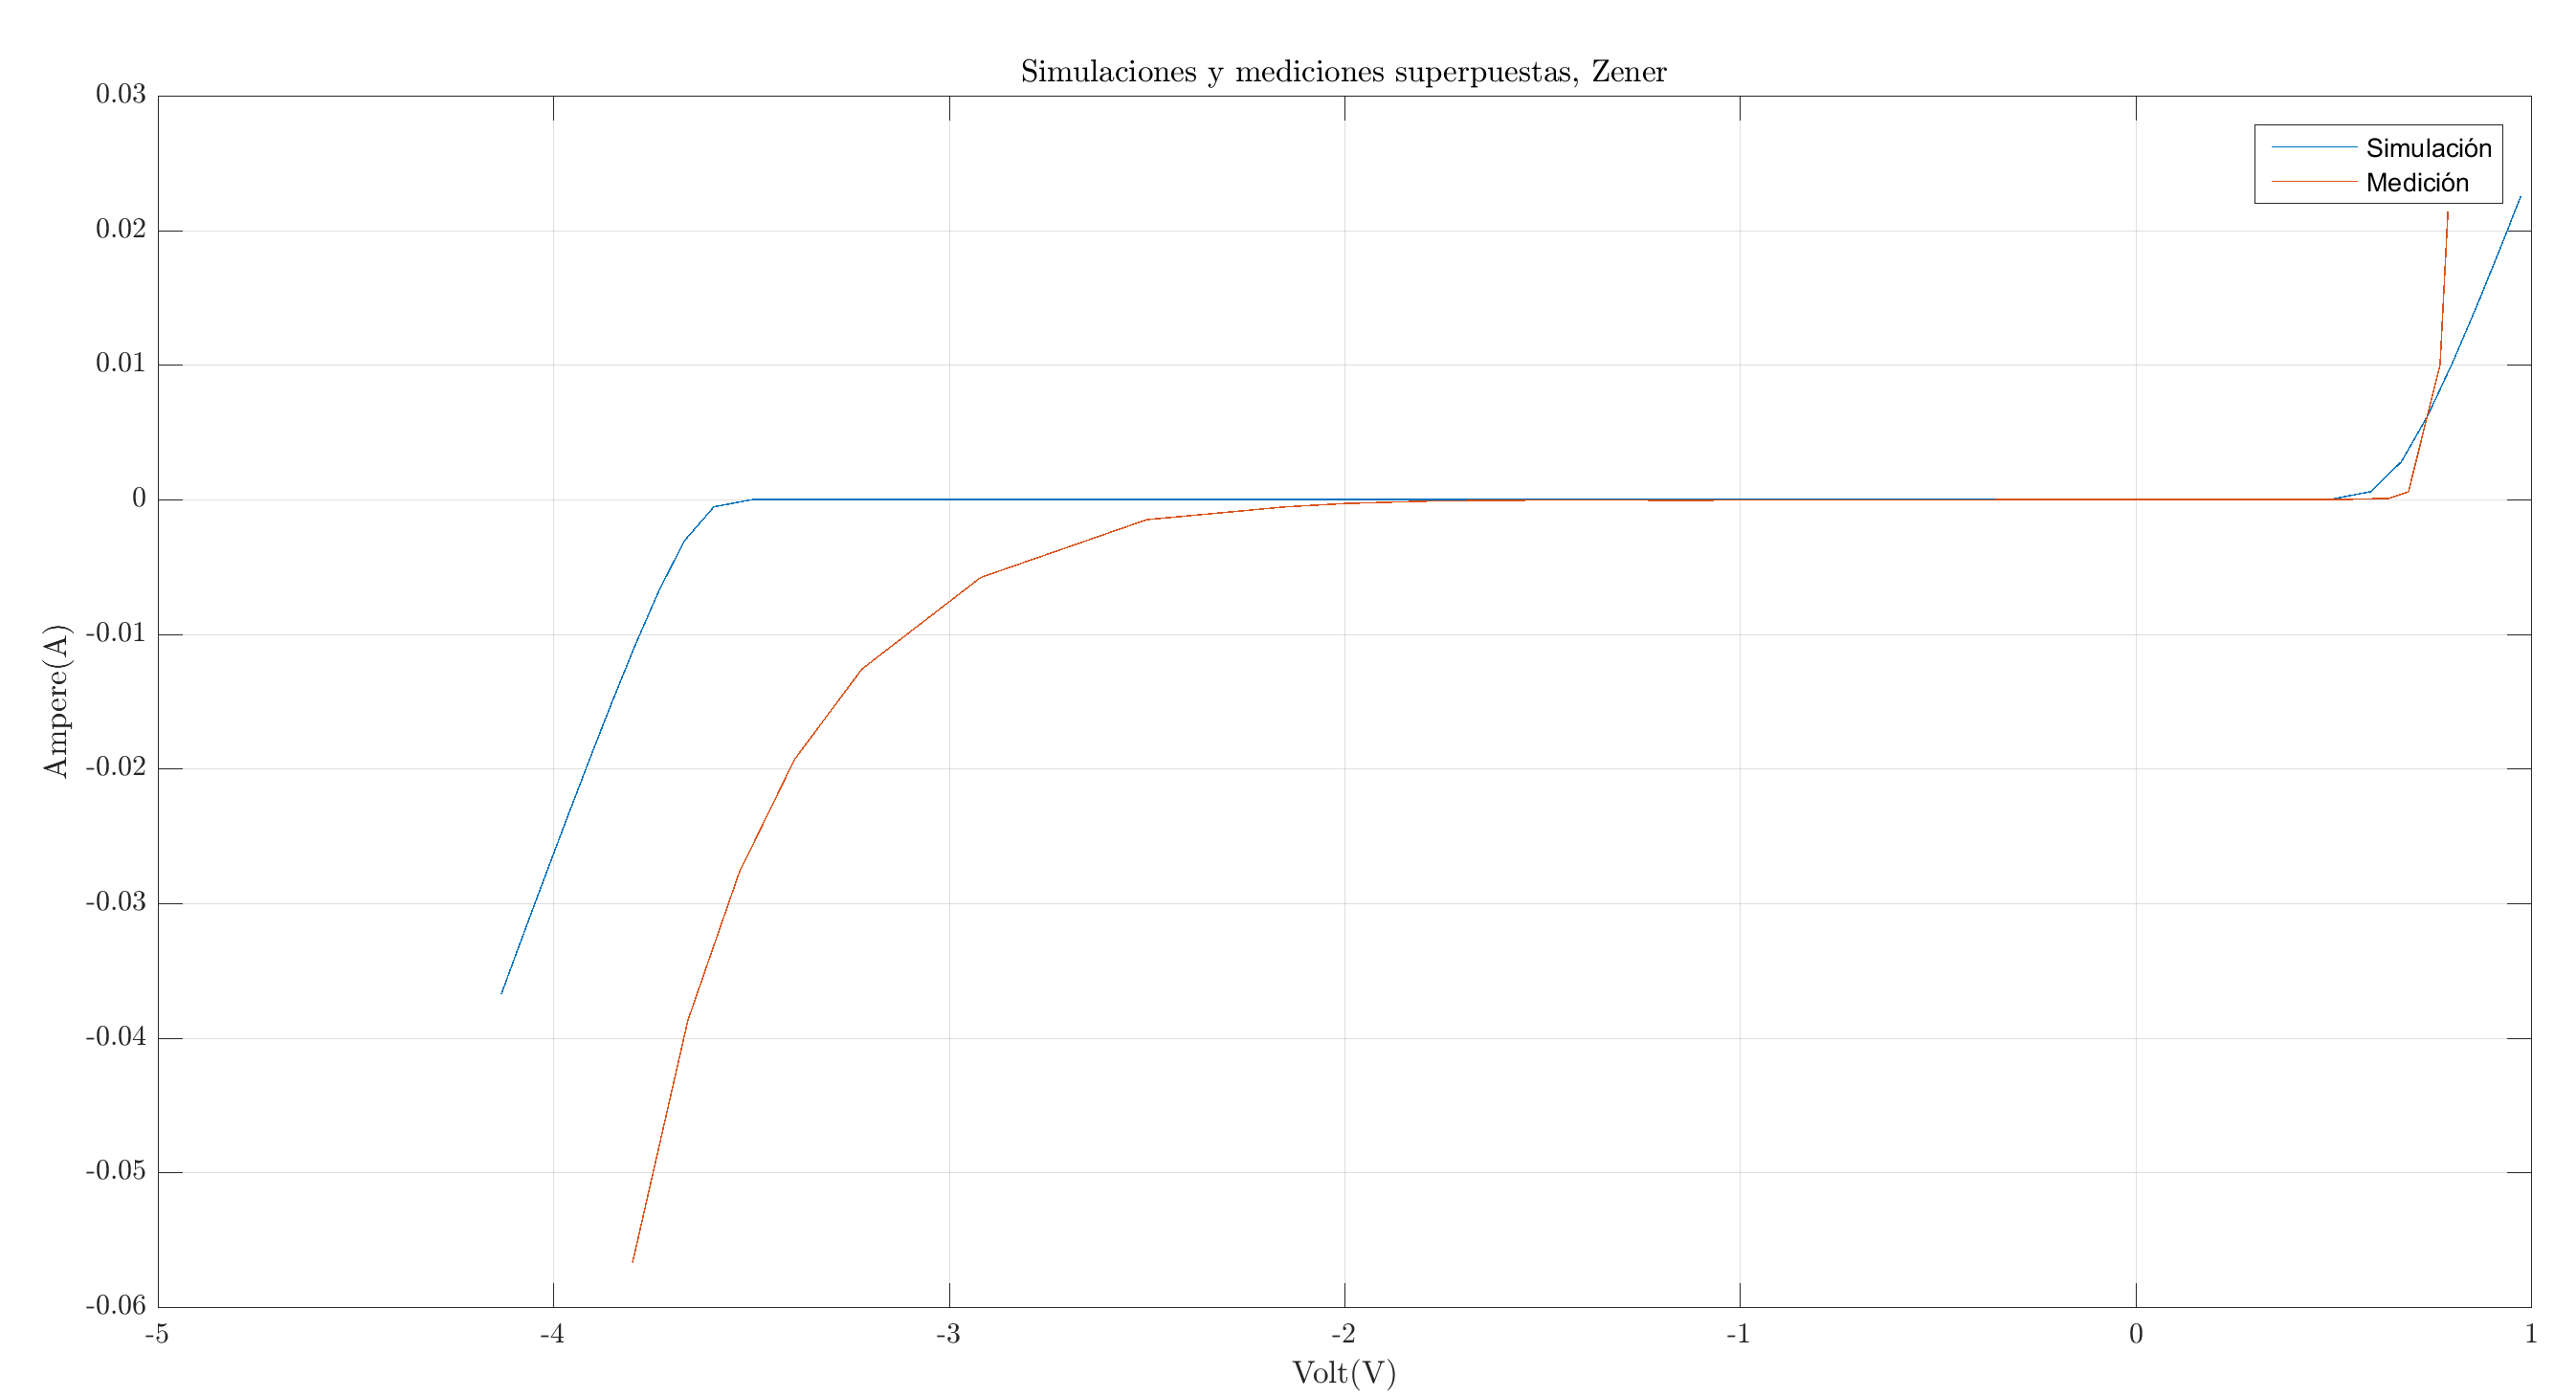
\includegraphics[scale=0.2]{imagenes/zener_simulacion_medicion.png}
	\caption{Simulación de la curva del zener y medición superpuestas.}
	\label{fig:ej5_zener_simulacion_medicion}
\end{figure}
	
	Como se puede notar, las curvas resultantes tienen la misma forma, la propia de un diodo zener, con una caída exponencial de la corriente cerca de la tensión de breakdown y una subida también exponencial para valores cercanos a 0.7V. Sin embargo, debe hacerse notar que la tensión a partir de la cual comienza la caída abrupta para la simulación es exactamente 3.9V, mientras que para el diodo medido, la caída comienza en valores cercanos a 2.5V.\par
	 La razón de esto se cree que es la diferencia de modelos elegidos para la simulación y para la medición, siendo el diodo 1N4730A con el que se contaba es un diodo de peor calidad, en el sentido en que el ''codo'' característico del zener comienza para valores de tensiones relativamente bajos, pero la caída abrupta comienza recién a partir de los 3.9V o valores cercanos a los mismos.\par 
	Debe recordarse de la sección anterior que los valores de medición de corriente nulos no necesariamente lo son así, sino que estos son los valores que pudo arrojar un un tester común en mínima escala, y que además se estima que las corrientes circulantes serán del orden de los \micro A. \par

\section{Curvas del transistor bipolar}

 El transistor utilizado fue un BC547. \par

 	El circuito propuesto para realizar las mediciones es el siguiente:

	\begin{figure}[H]	%transistor, circuito propuesto
		\centering
		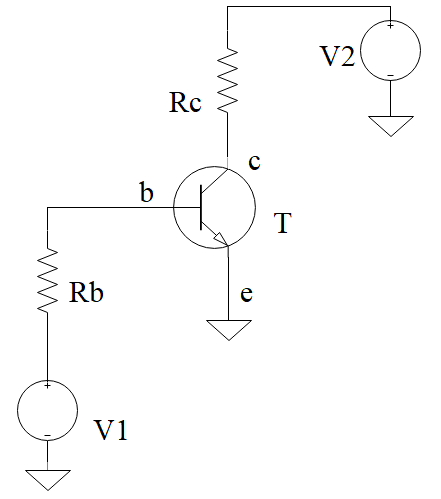
\includegraphics[scale=1.2]{imagenes/circuito_transistor.png}
		\caption{Circuito propuesto para las mediciones del transistor.}
		\label{fig:ej5_circuito_transistor}
	\end{figure}
	
	Los valores de resistencia elegidos fueron $R_B=33k\Omega$ y $R_C=150\Omega$: el primero para limitar la corriente de base a valores en el orden de los \micro A, y el segundo para poder observar los cambios en $V_{CE}$ en el rango de 30V de la fuente utilizada.\par
	Para cada curva, se asumió una corriente de base $I_b$ constante tanto al momento de simular como al de realizar las mediciones. Sin embargo, esto resulta ser una idealización, ya que en realidad la fuente de continua no podrá aportar una tensión exactamente igual para todos los valores de tensión entre colector y emisor. La tensión de la base también irá fluctuando y con eso también lo hará $I_b$. Se tomó un promedio de las corrientes de base para definir una curva a simular/medir.\par
	Resolviendo las mallas del circuito y asumiendo una caída de 0.7V sobre el transistor, se pudo definir el valor de tensión de la fuente de base para lograr cada corriente de base deseada y con ella trazar cada curva.\par
	Es así como, para una corriente de base fija, se realizó un barrido de tensión continua de $V_{2}$, con la cual se iba a su vez barriendo en tensi\'on emisor-colector, que se midi\'o tambi\'en utilizando un mult\'imetro.\par
	La corriente de base se midió a partir de tomar la tensión sobre la resistencia de base, cuyo valor era fijo y conocido. Análogamente, la corriente del colector se midió a partir de tomar la tensión sobre la resistencia del colector.\par
	
	Las curvas resultantes de las mediciones y de las simulaciones fueron las siguientes:	
	
		\begin{figure}[H]	%transistor, circuito propuesto
		\centering
		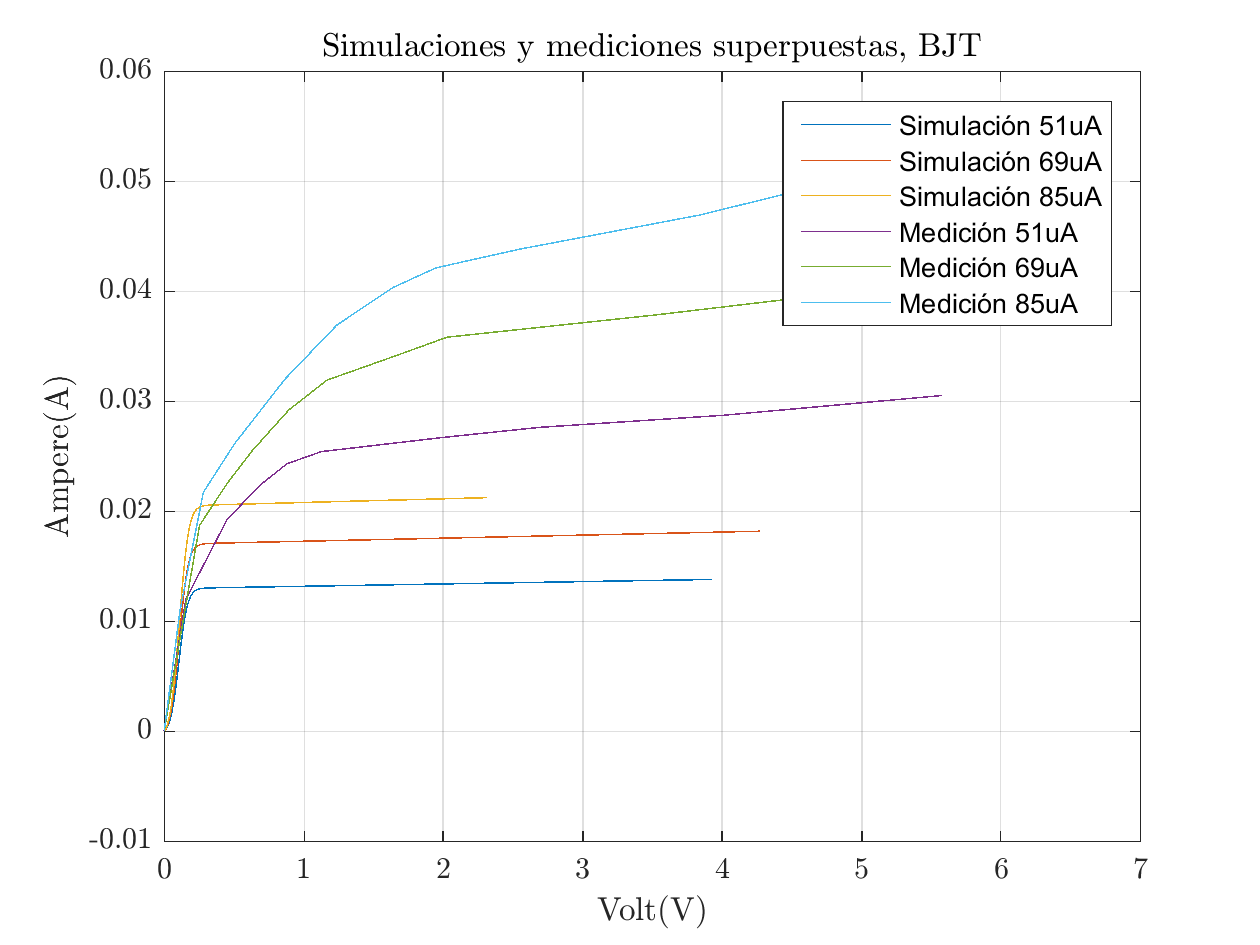
\includegraphics[scale=0.4]{imagenes/transistor_simulacion_medicion.png}
		\caption{Simulación de la curva del transistor y medición superpuestas.}
		\label{fig:ej5_transistor_simulacion_medicion}
	\end{figure}
	
	Si bien las curvas medidas respetan la forma general que esperaba obtenerse, se observan significantes discrepancias con la simulaci\'on. \par
	Para empezar, el valor de $I_{C}$ para el que la corriente comienza a depender de manera aproximadamente lineal de $V_{CE}$ es mucho menor en la simulaci\'on. Esto puede deberse a la gran dispresi\'on del valor de $h_{fe}$, que el fabricante s\'olo indica que se encuentra entre 110 y 800 (adimensional). La relaci\'on entre $I_C$ e $I_B$ indicar\'ia que LTSPICE considera $hfe \sim 250$, lo cual es mucho menor que el medido con el tester de 569. Con este \'ultimo $h_{fe}$ se pueden explicar las corrientes obtenidas para polarizaci\'on activa directa.  \par
	Por otro lado, en la simulaci\'on las curvas llegan a su comportamiento lineal para valores de $V_{CE}$ menores que para las mediciones. Aqu\'i pueden estar entrando en juego comportamentos no ideales del transistor no contemplados por el simulador, as\'i como otras diferencias entre el modelo gen\'erico y el transistor concreto que se utiliz\'o.

\end{document}
